% Options for packages loaded elsewhere
\PassOptionsToPackage{unicode}{hyperref}
\PassOptionsToPackage{hyphens}{url}
\PassOptionsToPackage{dvipsnames,svgnames,x11names}{xcolor}
%
\documentclass[
  letterpaper,
  DIV=11,
  numbers=noendperiod]{scrartcl}

\usepackage{amsmath,amssymb}
\usepackage{iftex}
\ifPDFTeX
  \usepackage[T1]{fontenc}
  \usepackage[utf8]{inputenc}
  \usepackage{textcomp} % provide euro and other symbols
\else % if luatex or xetex
  \usepackage{unicode-math}
  \defaultfontfeatures{Scale=MatchLowercase}
  \defaultfontfeatures[\rmfamily]{Ligatures=TeX,Scale=1}
\fi
\usepackage{lmodern}
\ifPDFTeX\else  
    % xetex/luatex font selection
\fi
% Use upquote if available, for straight quotes in verbatim environments
\IfFileExists{upquote.sty}{\usepackage{upquote}}{}
\IfFileExists{microtype.sty}{% use microtype if available
  \usepackage[]{microtype}
  \UseMicrotypeSet[protrusion]{basicmath} % disable protrusion for tt fonts
}{}
\makeatletter
\@ifundefined{KOMAClassName}{% if non-KOMA class
  \IfFileExists{parskip.sty}{%
    \usepackage{parskip}
  }{% else
    \setlength{\parindent}{0pt}
    \setlength{\parskip}{6pt plus 2pt minus 1pt}}
}{% if KOMA class
  \KOMAoptions{parskip=half}}
\makeatother
\usepackage{xcolor}
\setlength{\emergencystretch}{3em} % prevent overfull lines
\setcounter{secnumdepth}{-\maxdimen} % remove section numbering
% Make \paragraph and \subparagraph free-standing
\ifx\paragraph\undefined\else
  \let\oldparagraph\paragraph
  \renewcommand{\paragraph}[1]{\oldparagraph{#1}\mbox{}}
\fi
\ifx\subparagraph\undefined\else
  \let\oldsubparagraph\subparagraph
  \renewcommand{\subparagraph}[1]{\oldsubparagraph{#1}\mbox{}}
\fi


\providecommand{\tightlist}{%
  \setlength{\itemsep}{0pt}\setlength{\parskip}{0pt}}\usepackage{longtable,booktabs,array}
\usepackage{calc} % for calculating minipage widths
% Correct order of tables after \paragraph or \subparagraph
\usepackage{etoolbox}
\makeatletter
\patchcmd\longtable{\par}{\if@noskipsec\mbox{}\fi\par}{}{}
\makeatother
% Allow footnotes in longtable head/foot
\IfFileExists{footnotehyper.sty}{\usepackage{footnotehyper}}{\usepackage{footnote}}
\makesavenoteenv{longtable}
\usepackage{graphicx}
\makeatletter
\def\maxwidth{\ifdim\Gin@nat@width>\linewidth\linewidth\else\Gin@nat@width\fi}
\def\maxheight{\ifdim\Gin@nat@height>\textheight\textheight\else\Gin@nat@height\fi}
\makeatother
% Scale images if necessary, so that they will not overflow the page
% margins by default, and it is still possible to overwrite the defaults
% using explicit options in \includegraphics[width, height, ...]{}
\setkeys{Gin}{width=\maxwidth,height=\maxheight,keepaspectratio}
% Set default figure placement to htbp
\makeatletter
\def\fps@figure{htbp}
\makeatother

\usepackage{booktabs}
\usepackage{caption}
\usepackage{longtable}
\usepackage{colortbl}
\usepackage{array}
\usepackage{anyfontsize}
\usepackage{multirow}
\KOMAoption{captions}{tableheading}
\makeatletter
\makeatother
\makeatletter
\makeatother
\makeatletter
\@ifpackageloaded{caption}{}{\usepackage{caption}}
\AtBeginDocument{%
\ifdefined\contentsname
  \renewcommand*\contentsname{Table of contents}
\else
  \newcommand\contentsname{Table of contents}
\fi
\ifdefined\listfigurename
  \renewcommand*\listfigurename{List of Figures}
\else
  \newcommand\listfigurename{List of Figures}
\fi
\ifdefined\listtablename
  \renewcommand*\listtablename{List of Tables}
\else
  \newcommand\listtablename{List of Tables}
\fi
\ifdefined\figurename
  \renewcommand*\figurename{Figure}
\else
  \newcommand\figurename{Figure}
\fi
\ifdefined\tablename
  \renewcommand*\tablename{Table}
\else
  \newcommand\tablename{Table}
\fi
}
\@ifpackageloaded{float}{}{\usepackage{float}}
\floatstyle{ruled}
\@ifundefined{c@chapter}{\newfloat{codelisting}{h}{lop}}{\newfloat{codelisting}{h}{lop}[chapter]}
\floatname{codelisting}{Listing}
\newcommand*\listoflistings{\listof{codelisting}{List of Listings}}
\makeatother
\makeatletter
\@ifpackageloaded{caption}{}{\usepackage{caption}}
\@ifpackageloaded{subcaption}{}{\usepackage{subcaption}}
\makeatother
\makeatletter
\@ifpackageloaded{tcolorbox}{}{\usepackage[skins,breakable]{tcolorbox}}
\makeatother
\makeatletter
\@ifundefined{shadecolor}{\definecolor{shadecolor}{rgb}{.97, .97, .97}}
\makeatother
\makeatletter
\makeatother
\makeatletter
\makeatother
\ifLuaTeX
  \usepackage{selnolig}  % disable illegal ligatures
\fi
\IfFileExists{bookmark.sty}{\usepackage{bookmark}}{\usepackage{hyperref}}
\IfFileExists{xurl.sty}{\usepackage{xurl}}{} % add URL line breaks if available
\urlstyle{same} % disable monospaced font for URLs
\hypersetup{
  pdftitle={Text Analysis for SOcial Scientists and Leaders},
  colorlinks=true,
  linkcolor={blue},
  filecolor={Maroon},
  citecolor={Blue},
  urlcolor={Blue},
  pdfcreator={LaTeX via pandoc}}

\title{Text Analysis for SOcial Scientists and Leaders}
\usepackage{etoolbox}
\makeatletter
\providecommand{\subtitle}[1]{% add subtitle to \maketitle
  \apptocmd{\@title}{\par {\large #1 \par}}{}{}
}
\makeatother
\subtitle{Problem Set-1}
\author{Ilayda, Mithilesh and Bikash}
\date{}

\begin{document}
\maketitle
\ifdefined\Shaded\renewenvironment{Shaded}{\begin{tcolorbox}[boxrule=0pt, sharp corners, borderline west={3pt}{0pt}{shadecolor}, enhanced, frame hidden, breakable, interior hidden]}{\end{tcolorbox}}\fi

In Part 2 of the provided code, you learned how to build an ngram model
to predict the price of different restaurants. You split your data in
two. You trained a model to predict restaurant price in one half, and
tested the model's accuracy in the other half. You also plotted the
coefficients from the model. For the next three questions, complete the
exact same workflow for one other quantity of interest. You are allowed
to build a model to detect either gender (look for the ``male''
variable) or star rating (look for the ``stars'' variable). The choice
is up to you!

\hypertarget{produce-a-plot-showing-the-frequencies-and-coefficients-of-the-features-in-your-model.-makesure-it-is-easy-to-read}{%
\subsubsection{1. Produce a plot showing the frequencies and
coefficients of the features in your model. Makesure it is easy to
read!}\label{produce-a-plot-showing-the-frequencies-and-coefficients-of-the-features-in-your-model.-makesure-it-is-easy-to-read}}

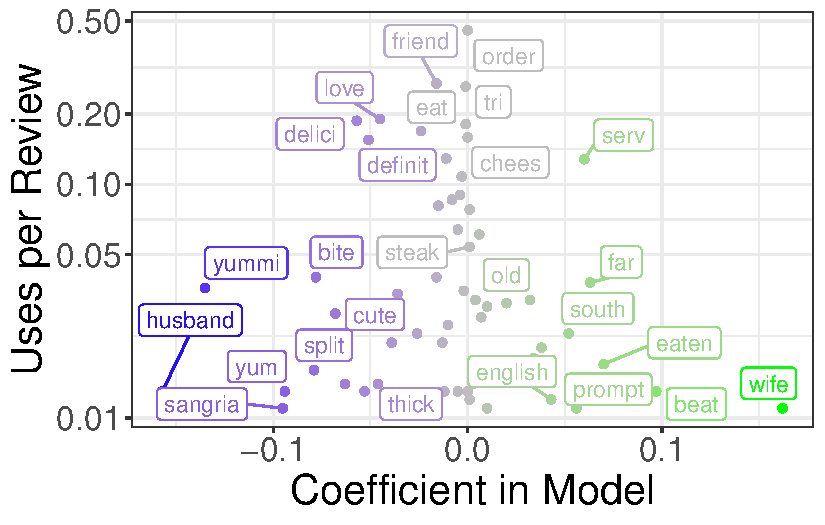
\includegraphics{nlp_ps_1_files/figure-pdf/unnamed-chunk-1-1.pdf}

\hypertarget{report-the-percentage-accuracy-of-the-model-you-trained-using-the-held-out-data-and-write-a-few-sentences-interpreting-the-results.-what-features-seemed-to-be-the-best-predictors-how-do-you-think-you-could-improve-the-model}{%
\subsubsection{1. Report the percentage accuracy of the model you
trained, using the held-out data, and write a few sentences interpreting
the results. What features seemed to be the best predictors? How do you
think you could improve the
model?}\label{report-the-percentage-accuracy-of-the-model-you-trained-using-the-held-out-data-and-write-a-few-sentences-interpreting-the-results.-what-features-seemed-to-be-the-best-predictors-how-do-you-think-you-could-improve-the-model}}

The model accuracy is 58.43\%. The best predictor turns out to be
whether reviewer mentions about his/her partner in the review.
Therefore, if you mention your wife in your reviews, the review is more
likely to written by the husband. We could improve this model by using
bi-grams or a combination of n-grams.

\begingroup
\fontsize{12.0pt}{14.4pt}\selectfont
\begin{longtable*}{lccc}
\toprule
 & \multicolumn{2}{c}{\textbf{Model Predictions}} &  \\ 
\cmidrule(lr){2-3}
 & Female & Male & \textbf{Total} \\ 
\midrule\addlinespace[2.5pt]
{\bfseries Actual Gender} &  &  &  \\ 
    Female & 482 (34\%) & 346 (24\%) & 828 (58\%) \\ 
    Male & 227 (16\%) & 362 (26\%) & 589 (42\%) \\ 
{\bfseries Total} & 709 (50\%) & 708 (50\%) & 1,417 (100\%) \\ 
\bottomrule
\end{longtable*}
\endgroup



\end{document}
